\documentclass[zihao=5,a4paper,UTF8]{ctexart}
\usepackage[top=2.0cm, bottom=2.0cm, left=2.0cm, right=2.0cm]{geometry}
\usepackage{amsmath, amssymb}
\usepackage{array, booktabs}
\usepackage{enumitem}
\usepackage{tikz}
\usepackage{fancyhdr}

\pagestyle{fancy}
\fancyhf{}
\fancyfoot[C]{\small 第 \thepage\ 页}
\renewcommand{\headrulewidth}{0pt}

\newcommand{\blank}[1][2.5cm]{\underline{\hspace{#1}}}
\newcommand{\choicebox}{\hfill(\hspace{1.8em})}

\begin{document}

\begin{center}
    {\Large\bfseries 南京航空航天大学}\\[4pt]
    {\large 2019 $\sim$ 2020 学年\ 第 1 学期\ 《大学物理 I(2)》考试试题}
\end{center}

\begin{center}
\begin{tabular}{|c|c|c|c|c|}
\hline
题号 & 一（30分） & 二（36分） & 三（34分） & 总分 \\
\hline
得分 & \hspace{2.2cm} & \hspace{2.2cm} & \hspace{2.2cm} & \hspace{2.2cm} \\
\hline
\end{tabular}
\end{center}

\section*{一、选择题（每题 3 分，共 30 分）}

\begin{enumerate}[leftmargin=2em, itemsep=6pt]
    \item 一质点作简谐振动，周期为 $T$，当它由平衡位置向 $x$ 轴正方向运动时，从二分之一最大位移处到最大位移处这段距离所经历的时间是\choicebox\\
    (A) $T/12$\qquad (B) $T/8$\qquad (C) $T/6$\qquad (D) $T/4$

    \item 右图为沿 $x$ 轴负方向传播的平面简谐波在 $t=0$ 时刻的波形，若波的表达式以余弦函数表示，则 $O$ 点处质点振动的初相为\choicebox\\
    \begin{minipage}[t]{0.68\textwidth}
    (A) $0$\qquad (B) $\pi/2$\qquad (C) $\pi$\qquad (D) $3\pi/2$
    \end{minipage}%
    \begin{minipage}[t]{0.30\textwidth}
    \centering
    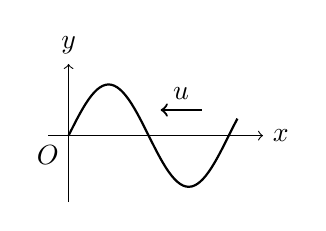
\begin{tikzpicture}[scale=0.65, baseline=(current bounding box.north)]
        \draw[->] (-0.4,0) -- (3.8,0) node[right] {$x$};
        \draw[->] (0,-1.3) -- (0,1.4) node[above] {$y$};
        \draw[thick, domain=0:3.3, samples=60] plot (\x, {sin(115*\x)});
        \draw[->, thick] (2.6,0.5) -- (1.8,0.5) node[midway,above] {$u$};
        \node[below left] at (0,0) {$O$};
    \end{tikzpicture}
    \end{minipage}

    \item 下图中画出一向右传播的简谐波在 $t$ 时刻的波形图，$MN$ 为波密介质的反射面，发生全反射，则反射波在 $t$ 时刻的波形图（下图右）为\choicebox\\
    \begin{center}
    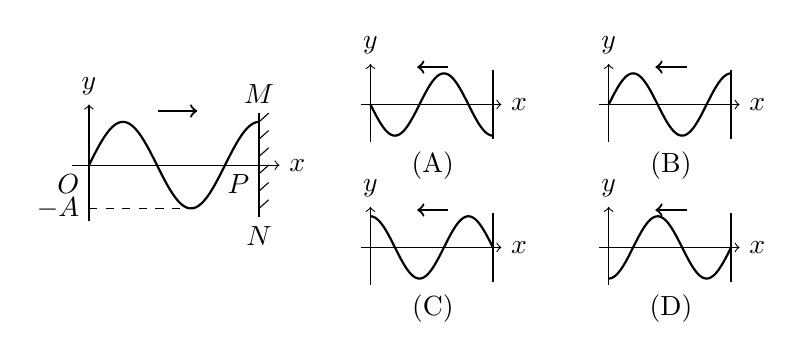
\begin{tikzpicture}[scale=0.55]
        % 入射波
        \draw[->] (-0.4,0) -- (4.4,0) node[right] {$x$};
        \draw[->] (0,-1.3) -- (0,1.4) node[above] {$y$};
        \draw[thick, domain=0:3.927, samples=60] plot (\x, {sin(180*\x/1.5708)});
        \draw[->, thick] (1.6,1.25) -- (2.5,1.25);
        \draw[thick] (3.927,-1.2) -- (3.927,1.2);
        \foreach \y in {-1.0,-0.6,-0.2,0.2,0.6,1.0} {\draw (3.927,\y) -- (4.15,\y+0.2);}
        \node[above] at (3.927,1.2) {$M$};
        \node[below] at (3.927,-1.2) {$N$};
        \node[below left] at (0,0) {$O$};
        \node[below left] at (3.927,0) {$P$};
        \node[left] at (0,-1) {$-A$};
        \draw[dashed] (0,-1) -- (2.35,-1);
        % 选项 A
        \begin{scope}[xshift=6.5cm, yshift=1.4cm, scale=0.72]
            \draw[->] (-0.3,0) -- (4.2,0) node[right] {$x$};
            \draw[->] (0,-1.2) -- (0,1.3) node[above] {$y$};
            \draw[thick, domain=0:3.927, samples=50] plot (\x, {-sin(180*\x/1.5708)});
            \draw[->, thick] (2.5,1.2) -- (1.5,1.2);
            \draw[thick] (3.927,-1.1) -- (3.927,1.1);
            \node[below] at (2,-1.2) {(A)};
        \end{scope}
        % 选项 B
        \begin{scope}[xshift=12.0cm, yshift=1.4cm, scale=0.72]
            \draw[->] (-0.3,0) -- (4.2,0) node[right] {$x$};
            \draw[->] (0,-1.2) -- (0,1.3) node[above] {$y$};
            \draw[thick, domain=0:3.927, samples=50] plot (\x, {sin(180*\x/1.5708)});
            \draw[->, thick] (2.5,1.2) -- (1.5,1.2);
            \draw[thick] (3.927,-1.1) -- (3.927,1.1);
            \node[below] at (2,-1.2) {(B)};
        \end{scope}
        % 选项 C
        \begin{scope}[xshift=6.5cm, yshift=-1.9cm, scale=0.72]
            \draw[->] (-0.3,0) -- (4.2,0) node[right] {$x$};
            \draw[->] (0,-1.2) -- (0,1.3) node[above] {$y$};
            \draw[thick, domain=0:3.927, samples=50] plot (\x, {cos(180*\x/1.5708)});
            \draw[->, thick] (2.5,1.2) -- (1.5,1.2);
            \draw[thick] (3.927,-1.1) -- (3.927,1.1);
            \node[below] at (2,-1.2) {(C)};
        \end{scope}
        % 选项 D
        \begin{scope}[xshift=12.0cm, yshift=-1.9cm, scale=0.72]
            \draw[->] (-0.3,0) -- (4.2,0) node[right] {$x$};
            \draw[->] (0,-1.2) -- (0,1.3) node[above] {$y$};
            \draw[thick, domain=0:3.927, samples=50] plot (\x, {-cos(180*\x/1.5708)});
            \draw[->, thick] (2.5,1.2) -- (1.5,1.2);
            \draw[thick] (3.927,-1.1) -- (3.927,1.1);
            \node[below] at (2,-1.2) {(D)};
        \end{scope}
    \end{tikzpicture}
    \end{center}

    \item 图示一平面简谐机械波在 $t$ 时刻的波形曲线，若此时 $A$ 点处媒质质元的振动动能在增大，则\choicebox\\
    \begin{minipage}[t]{0.68\textwidth}
    (A) $A$ 点处质元的弹性势能在减小；\\
    (B) 波沿 $x$ 轴负方向传播；\\
    (C) $B$ 点处质元的振动动能在减小；\\
    (D) 各点波的能量密度都不随时间变化。
    \end{minipage}%
    \begin{minipage}[t]{0.30\textwidth}
    \centering
    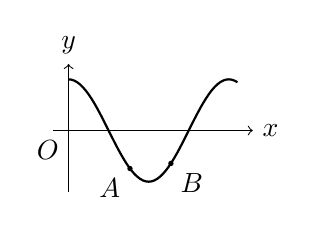
\begin{tikzpicture}[scale=0.65, baseline=(current bounding box.north)]
        \draw[->] (-0.3,0) -- (3.6,0) node[right] {$x$};
        \draw[->] (0,-1.2) -- (0,1.3) node[above] {$y$};
        \draw[thick, domain=0:3.3, samples=60] plot (\x, {cos(115*\x)});
        \fill (1.2,{cos(115*1.2)}) circle (1.5pt) node[below left] {$A$};
        \fill (2.0,{cos(115*2.0)}) circle (1.5pt) node[below right] {$B$};
        \node[below left] at (0,0) {$O$};
    \end{tikzpicture}
    \end{minipage}

    \item 在相同的时间内，一束波长为 $\lambda$ 的单色光在空气中和在玻璃中\choicebox\\
    (A) 传播的路程相等，走过的光程相等；\qquad (B) 传播的路程相等，走过的光程不相等；\\
    (C) 传播的路程不相等，走过的光程相等；\qquad (D) 传播的路程不相等，走过的光程不相等。

    \item 在如图所示的单缝夫琅禾费衍射实验中，若将单缝沿透镜光轴方向向透镜平移，则屏幕上的衍射条纹\choicebox\\
    \begin{minipage}[t]{0.65\textwidth}
    (A) 间距变大；\qquad (B) 间距变小；\\
    (C) 不发生变化；\qquad (D) 间距不变，但明暗条纹的位置交替变化。
    \end{minipage}%
    \begin{minipage}[t]{0.32\textwidth}
    \centering
    \begin{tikzpicture}[scale=0.55, baseline=(current bounding box.north)]
        \draw[thick] (0,0.4) -- (0,1.2) (0,-0.4) -- (0,-1.2);
        \draw[->] (-1,0.2) -- (-0.2,0.2);
        \draw[->] (-1,-0.2) -- (-0.2,-0.2);
        \draw[dashed] (-1.2,0) -- (3.5,0);
        \draw[thick] (1.3,0) ellipse (0.15 and 1.1);
        \node[above] at (1.3,1.1) {$L$};
        \draw[thick] (3.3,-1.2) -- (3.3,1.2) node[above] {屏幕};
        \draw[<->] (1.3,-1.0) -- (3.3,-1.0) node[midway,below] {$f$};
    \end{tikzpicture}
    \end{minipage}

    \item 在狭义相对论中，下列说法中哪些是正确的？\choicebox\\
    (1) 一切运动物体相对于观察者的速度都不能大于真空中的光速；\\
    (2) 质量、长度、时间的测量结果都是随物体与观察者的相对运动状态而发生改变的；\\
    (3) 在一惯性系中发生于同一时刻、不同地点的两个事件在其它一切惯性系中也是同时发生的；\\
    (4) 惯性系中的观察者观察一个与他作匀速相对运动的时钟时，会看到这时钟比与他相对静止的相同的时钟走得慢些。\\
    (A) (1), (3), (4)\qquad (B) (1), (2), (4)\qquad (C) (1), (2), (3)\qquad (D) (2), (3), (4)

    \item 电子显微镜中的电子从静止开始通过电势差为 $U$ 的静电场加速后，其德布罗意波长是 $0.04\ \mathrm{nm}$，则 $U$ 约为（$h=6.63\times 10^{-34}\ \mathrm{J\cdot s}$，$e=1.6\times 10^{-19}\ \mathrm{C}$，$m_e=0.91\times 10^{-30}\ \mathrm{kg}$）\choicebox\\
    (A) $150\ \mathrm{V}$\qquad (B) $200\ \mathrm{V}$\qquad (C) $660\ \mathrm{V}$\qquad (D) $940\ \mathrm{V}$

    \item 用强度为 $I$、波长为 $\lambda$ 的 X 射线分别照射锂（原子序数 $Z=3$）和铁（$Z=26$），若在同一散射角下测得康普顿散射光的波长分别为 $\lambda_{\mathrm{Li}}$ 和 $\lambda_{\mathrm{Fe}}$，则\choicebox\\
    (A) $\lambda_{\mathrm{Li}} > \lambda_{\mathrm{Fe}}$\qquad (B) $\lambda_{\mathrm{Li}} < \lambda_{\mathrm{Fe}}$\qquad (C) $\lambda_{\mathrm{Li}} = \lambda_{\mathrm{Fe}}$\qquad (D) 无法比较

    \item 关于不确定关系 $\Delta p_x \Delta x \ge \hbar\ (\hbar = h/(2\pi))$，有以下几种理解：\\
    (1) 粒子的动量不可能确定；\qquad (2) 粒子的坐标不可能确定；\\
    (3) 粒子的动量和坐标不可能同时准确地确定；\qquad (4) 不确定关系不仅适用于电子和光子，也适用于其它粒子。\\
    其中正确的是：\choicebox\\
    (A) (1), (2)\qquad (B) (2), (4)\qquad (C) (3), (4)\qquad (D) (4), (1)
\end{enumerate}

\section*{二、填空题（共 36 分）}

\begin{enumerate}[leftmargin=2em, itemsep=6pt, start=11]
    \item 设平面简谐波沿 $x$ 轴传播时在 $x=0$ 处发生反射，反射波表达式为 $y_2 = A\cos\left[2\pi\left(\nu t - \frac{x}{\lambda}\right) + \frac{\pi}{2}\right]$。已知反射点为一自由端，则由入射波和反射波形成的驻波的波节位置的坐标为\blank[4.5cm]。

    \item \begin{minipage}[t]{0.72\textwidth}
    如图所示，双缝干涉实验装置中两个缝用厚度均为 $e$、折射率分别为 $n_1$ 和 $n_2$ 的透明介质膜覆盖（$n_1 > n_2$）。波长为 $\lambda$ 的平行单色光斜入射到双缝上，入射角为 $\theta$，双缝间距为 $d$，在屏幕中央 $O$ 处（$\overline{S_1O} = \overline{S_2O}$），两束相干光的相位差 $\Delta\phi = \blank[4.5cm]$。
    \end{minipage}%
    \begin{minipage}[t]{0.26\textwidth}
    \centering
    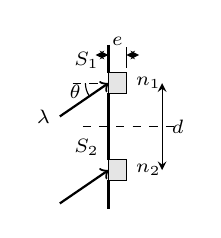
\begin{tikzpicture}[scale=0.65, baseline=(current bounding box.north)]
        % 挡板与双缝 S1, S2
        \draw[very thick] (0,1.6) -- (0,1.05);
        \draw[very thick] (0,0.65) -- (0,-0.65);
        \draw[very thick] (0,-1.05) -- (0,-1.6);
        % 介质膜 n1, n2
        \draw[fill=gray!20] (0,0.65) rectangle (0.35,1.05);
        \draw[fill=gray!20] (0,-1.05) rectangle (0.35,-0.65);
        \node[right] at (0.35,0.85) {\scriptsize $n_1$};
        \node[right] at (0.35,-0.85) {\scriptsize $n_2$};
        \node[above left] at (0,0.95) {\scriptsize $S_1$};
        \node[above left] at (0,-0.75) {\scriptsize $S_2$};
        % 厚度 e 标注
        \draw[thin] (0,1.15) -- (0,1.55);
        \draw[thin] (0.35,1.15) -- (0.35,1.55);
        \draw[<->, >=stealth, thin] (-0.25,1.4) -- (0,1.4);
        \draw[<->, >=stealth, thin] (0.6,1.4) -- (0.35,1.4);
        \node[above] at (0.175,1.4) {\scriptsize $e$};
        % 中心虚线与间距 d
        \draw[dashed] (-0.5,0) -- (1.4,0);
        \draw[dashed] (-0.7,0.85) -- (0,0.85);
        \draw[<->, >=stealth] (1.05,-0.85) -- (1.05,0.85) node[midway, right] {\scriptsize $d$};
        % 斜入射光
        \draw[->, thick] (-0.95,0.20) -- (0,0.85);
        \draw[->, thick] (-0.95,-1.50) -- (0,-0.85);
        \node[left] at (-0.95,0.20) {\scriptsize $\lambda$};
        \draw (-0.45,0.85) arc (180:214:0.45);
        \node at (-0.65,0.68) {\scriptsize $\theta$};
    \end{tikzpicture}
    \end{minipage}

    \item \begin{minipage}[t]{0.70\textwidth}
    $NN$ 为涂有极薄感光层的玻璃板，$MM$ 与 $NN$ 之间夹角 $\varphi = 3.0\times 10^{-4}\ \mathrm{rad}$，波长为 $\lambda$ 的平面单色光通过 $NN$ 板垂直入射到 $MM$ 金属反射镜上，则反射光与入射光在相遇区域形成光驻波，在 $NN$ 板的感光膜上形成对应于波腹波节的条纹，实验测得两个相邻的驻波波腹感光点 $A, B$ 的间距 $\overline{AB} = 1.0\ \mathrm{mm}$，则入射光波的波长 $\lambda$ 为\blank[2.5cm]$\mathrm{mm}$。
    \end{minipage}%
    \begin{minipage}[t]{0.28\textwidth}
    \centering
    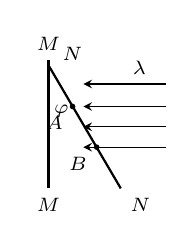
\begin{tikzpicture}[scale=0.68, baseline=(current bounding box.north)]
        % 金属反射镜 MM
        \draw[very thick] (0,-0.3) -- (0,2.1);
        \node[above] at (0,2.1) {\scriptsize $M$};
        \node[below] at (0,-0.3) {\scriptsize $M$};
        % 玻璃板 NN
        \draw[thick] (0,2.0) -- (1.35,-0.3);
        \node[above right] at (0.08,1.9) {\scriptsize $N$};
        \node[below right] at (1.35,-0.3) {\scriptsize $N$};
        \node at (0.24,1.15) {\scriptsize $\varphi$};
        % 点 A, B
        \fill (0.45,1.23) circle (1.5pt) node[below left] {\scriptsize $A$};
        \fill (0.90,0.47) circle (1.5pt) node[below left] {\scriptsize $B$};
        % 入射光
        \draw[<-, >=stealth] (0.65,1.65) -- (2.2,1.65);
        \draw[<-, >=stealth] (0.65,1.23) -- (2.2,1.23);
        \draw[<-, >=stealth] (0.65,0.85) -- (2.2,0.85);
        \draw[<-, >=stealth] (0.65,0.47) -- (2.2,0.47);
        \node[above] at (1.7,1.65) {\scriptsize $\lambda$};
    \end{tikzpicture}
    \end{minipage}

    \item 在牛顿环装置的平凸透镜和平玻璃板之间充满折射率 $n$ 的透明液体（设平凸透镜和平玻璃板的折射率都大于 $n$），凸透镜的曲率半径为 $R$，波长 $\lambda$ 的平行单色光垂直照射到牛顿环装置上，凸透镜顶部刚好与平玻璃板接触，则从中心向外数第十个明环所在处的液体厚度为 $e_{10} = \blank[2.8cm]$；第十个明环的半径 $r_{10} = \blank[2.8cm]$。

    \item 在单缝夫琅禾费衍射实验中，屏上第三级暗纹对应于单缝处波面可划分为\blank[2.0cm]个半波带，若将缝宽缩小一半，原来第三级暗纹处将是\blank[2.5cm]纹。

    \item 两个偏振片堆叠在一起，其偏振化方向相互垂直，若一束强度为 $I_0$ 的线偏振光入射，其光矢量振动方向与第一偏振片偏振化方向夹角为 $\pi/4$，则穿过第一偏振片后的光强为\blank[2.5cm]，穿过两个偏振片后的光强为\blank[2.5cm]。

    \item $A$、$B$ 两粒子的静止质量均为 $m_0$，其中 $A$ 静止，$B$ 以 $6m_0c^2$ 的动能与 $A$ 碰撞后合成为一个粒子且无能量释放，则复合粒子的静质量为\blank[2.5cm]。

    \item 设氢原子的动能等于氢原子处于温度为 $T$ 的热平衡状态时的平均动能，氢原子的质量为 $m_H$，那么此氢原子的德布罗意波长为\blank[3.5cm]。

    \item 爱因斯坦狭义相对论的两条基本原理是（需写出原理内容）：\blank[5cm]、\blank[5cm]。
\end{enumerate}

\section*{三、计算题（共 34 分）}

\begin{enumerate}[leftmargin=2em, itemsep=8pt, start=20]
    \item \begin{minipage}[t]{0.70\textwidth}
    （10 分）如图，一角频率为 $\omega_0$、振幅为 $A$ 的平面简谐波沿 $x$ 轴正方向传播，设在 $t=0$ 时该波在原点 $O$ 处引起的振动使该质元由平衡位置向 $y$ 轴负方向运动。$M$ 是垂直于 $x$ 轴的波密媒质反射面。已知 $\overline{OO'} = 7\lambda/4$，$\overline{PO'} = \lambda/4$（$\lambda$ 为波长），设反射波不衰减，求：\\
    （1）入射波与反射波的表达式；\\
    （2）$P$ 点的振动方程。
    \end{minipage}%
    \begin{minipage}[t]{0.28\textwidth}
    \centering
    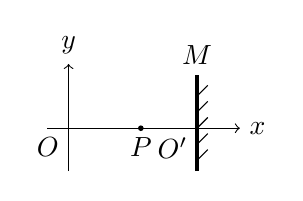
\begin{tikzpicture}[scale=0.68, baseline=(current bounding box.north)]
        \draw[->] (-0.4,0) -- (3.2,0) node[right] {$x$};
        \draw[->] (0,-0.8) -- (0,1.2) node[above] {$y$};
        \node[below left] at (0,0) {$O$};
        \fill (1.35,0) circle (1.5pt) node[below] {$P$};
        \draw[very thick] (2.4,-0.8) -- (2.4,1.0);
        \foreach \y in {-0.6,-0.3,0,0.3,0.6} {\draw (2.4,\y) -- (2.6,\y+0.2);}
        \node[above] at (2.4,1.0) {$M$};
        \node[below left] at (2.4,0) {$O'$};
    \end{tikzpicture}
    \end{minipage}

    \item （8 分）一双缝，缝距 $d=0.40\ \mathrm{mm}$，两缝宽度都是 $a=0.080\ \mathrm{mm}$，用波长为 $\lambda=480\ \mathrm{nm}$ 的平行光垂直照射双缝，在双缝后放一焦距 $f=2.0\ \mathrm{m}$ 的透镜，求：\\
    （1）在透镜焦平面处的屏上，双缝干涉条纹的间距 $l$；\\
    （2）在单缝衍射中央亮纹范围内的双缝干涉亮纹数目 $N$ 和相应的级数。

    \item （8 分）在 $K$ 惯性系中，相距 $\Delta x = 5\times 10^6\ \mathrm{m}$ 的两个地方发生两个事件，时间间隔 $\Delta t = 0.01\ \mathrm{s}$，而在相对于 $K$ 系沿 $x$ 正方向运动的 $K'$ 系中观察到这两个事件是同时发生的，求在 $K'$ 系中测量这两个事件的地点间隔是多少？

    \item （8 分）设质量为 $m$ 的微观粒子处在宽度为 $a$ 的一维无限深势阱中，试求：\\
    （1）粒子在 $0 \le x \le a/4$ 区间中出现的概率，并对 $n=1$ 和 $n=\infty$ 的情况算出概率值；\\
    （2）在哪些量子态上，$a/4$ 处的概率密度最大？\\
    （提示：粒子波函数为 $\psi_n(x) = \sqrt{\frac{2}{a}}\sin\frac{n\pi x}{a}$）
\end{enumerate}

\end{document}
